\section*{Exercício 1: Calculadora de Desconto}

\begin{enumerate}
    \item \textbf{Qual foi o primeiro teste criado?}
    
    O primeiro teste criado foi a função \texttt{test\_calcular\_desconto\_10()}, responsável por validar o desconto de 10\% sobre o valor de 100, esperando como resultado o valor 90.

    \item \textbf{Por que ele falhou?}
    
    O teste falhou por asserção (\textit{AssertionError}), pois na fase RED a função \texttt{calcular\_desconto(valor, percentual)} no módulo \texttt{calculadora.py} apenas definia um esqueleto de método com retorno \texttt{None}, resultando na falha \texttt{assert None == 90} mostrada pelo \textit{Pytest}.

    \begin{figure}[htbp]
        \centering
        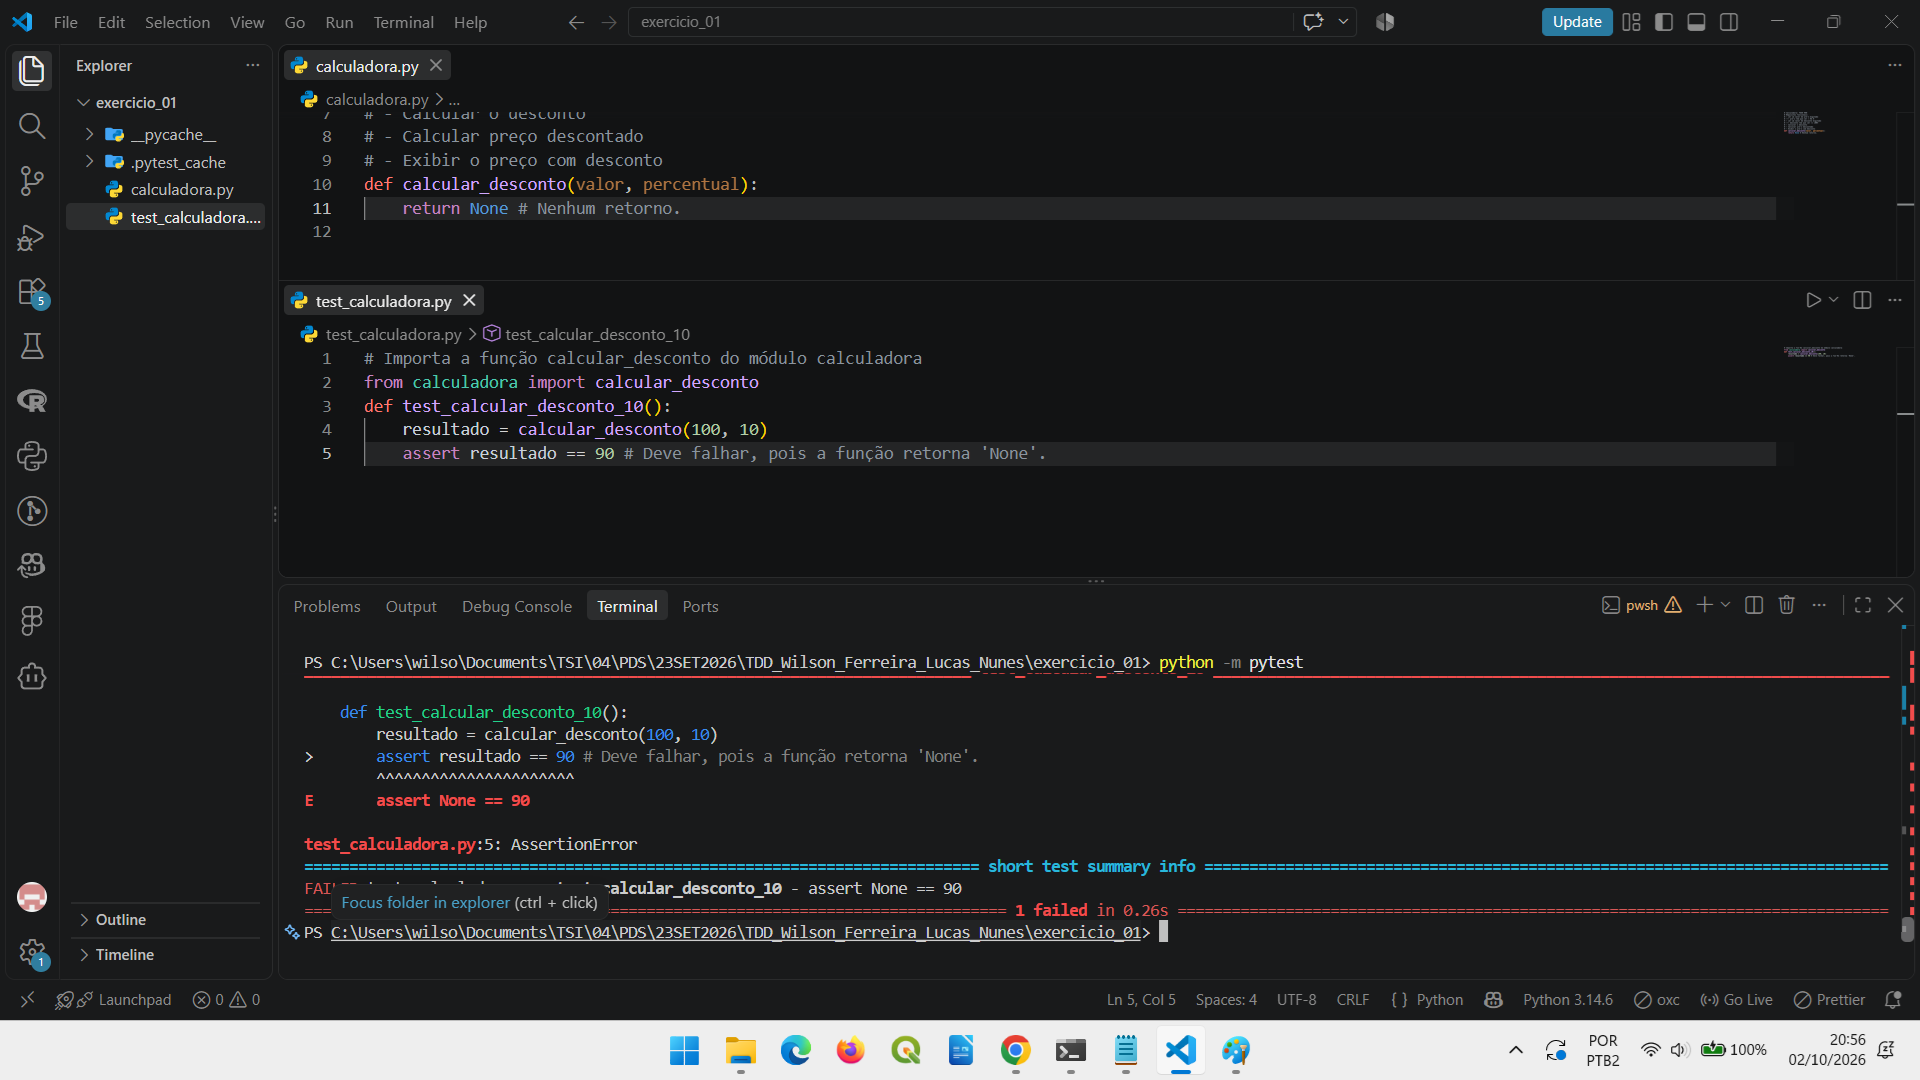
\includegraphics[width=0.92\textwidth]{ex01_red.png}
        \caption{Evidência da fase RED: falha de asserção no Pytest.}
        \label{fig:ex01_red}
    \end{figure}

    \item \textbf{Como você fez o teste passar?}
    
    A fórmula matemática mínima necessária foi implmentada em \texttt{calculadora.py}: o cálculo do valor final descontado através da expressão \texttt{valor * (1 - percentual / 100)}, satisfazendo a asserção e fazendo a execução verde no \textit{Pytest} (fase GREEN).

    \begin{figure}[htbp]
        \centering
        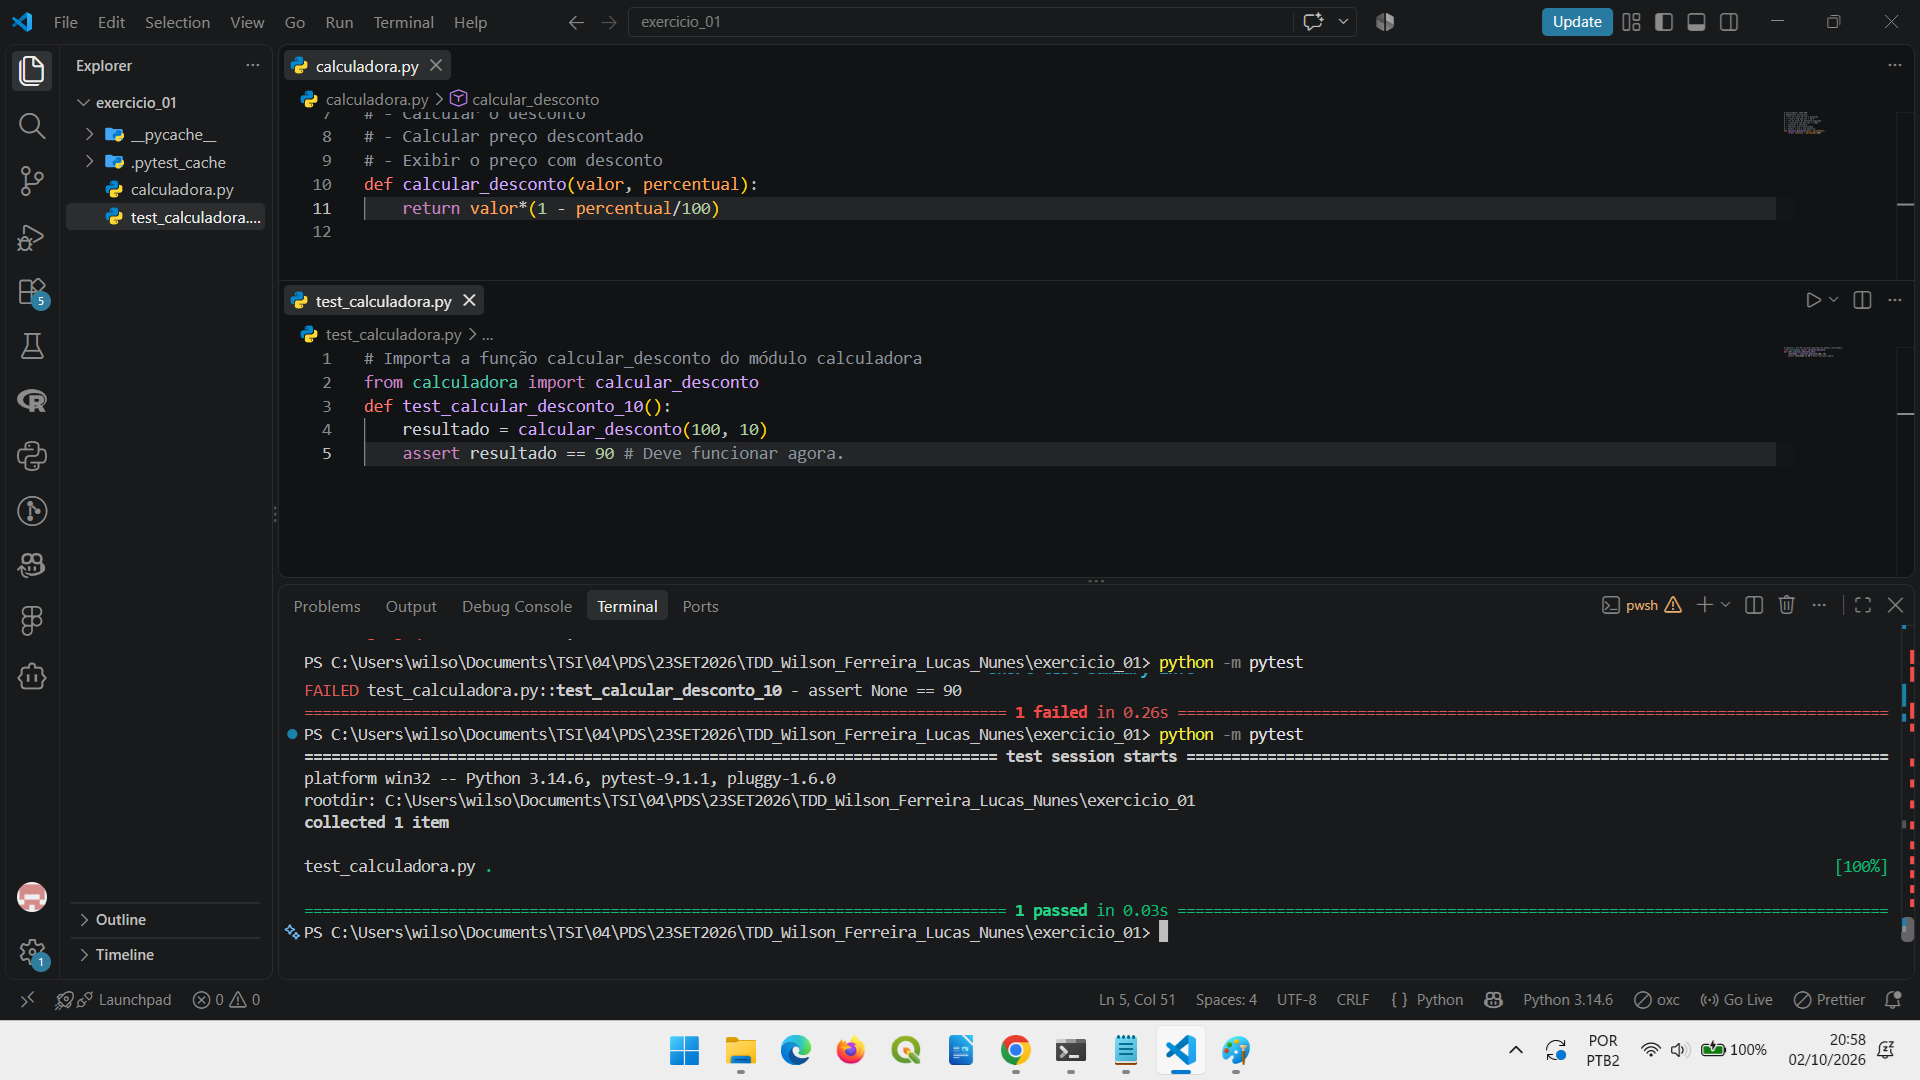
\includegraphics[width=0.92\textwidth]{ex01_green.png}
        \caption{Evidência da fase GREEN: teste obrigatório aprovado.}
        \label{fig:ex01_green}
    \end{figure}

    \item \textbf{O que foi alterado durante a refatoração?}
    
    Na fase REFACTOR, o conjunto de testes foi expandido para cobrir todos os cenários obrigatórios (20\%, 0\% e 100\%) da questão e os casos do desafio adicional (preço negativo e desconto superior a 100\%). Em \texttt{calculadora.py}, foram adicionadas condições de guarda com lançamento de exceções  (\texttt{raise ValueError}), validadas via \texttt{pytest.raises(ValueError)}, confirmando  os 6 testes passando normalmente.

    \begin{figure}[htbp]
        \centering
        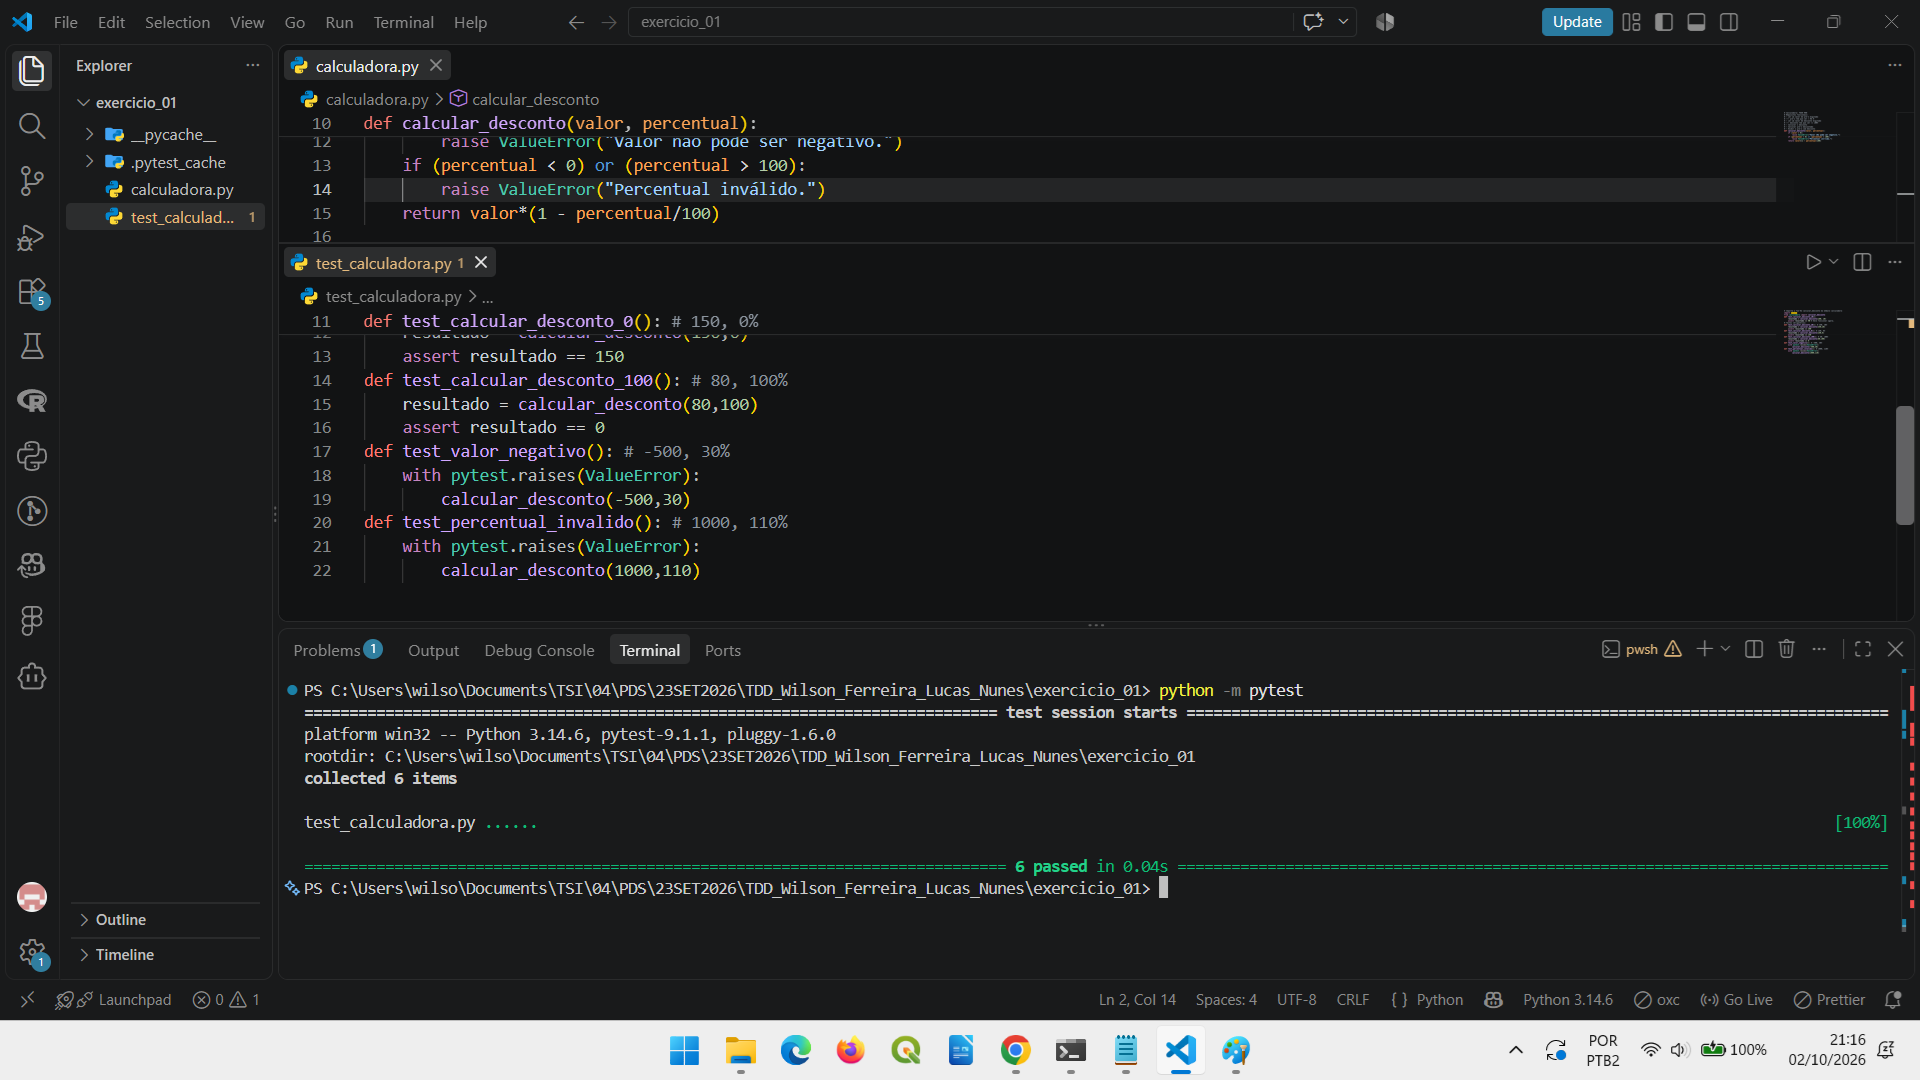
\includegraphics[width=0.92\textwidth]{ex01_refactor.png}
        \caption{Evidência da fase REFACTOR: 6 testes aprovados.}
        \label{fig:ex01_refactor}
    \end{figure}
\end{enumerate}